\section{Environmental noise}

Environmental noise refers to any signal originating from outside the structure of a \ac{GW} detector that can impact the detector's sensitivity or disrupt its ability to achieve and maintain lock.
The effects of environmental noise on detector sensitivity can range from persistent excess noise in the \ac{GW} strain data, to short-duration transient signals, or \textit{glitches}.

One goal of studying environmental noise is to aid in the validation of \ac{GW} events.
Due to the sophisticated nature of the search pipelines used to detect gravitational waves in the \ac{LIGO} data, environmental glitches are highly unlikely to fully account for a \ac{GW} event candidate.
That said, glitches capable of influencing analyses occur frequently at both observatories.

Unlike instrumental noise, environmental noise can potentially be correlated between different detectors, i.e. stemming from a common source as opposed to stemming from chance coincidence.
Such correlated noise is not accounted for in the estimation of false-alarm probabilities, which is done by time-shifting background data from each \ac{LIGO} detector to produce long stretches of coincident background.

Environmental noise is particularly important in searches for un-modeled sources of gravitational waves, as these look for excess power without the use of waveform templates.
Even for highly significant \ac{CBC} events, contamination of the strain data can be detrimental to parameter estimation analyses that infer source properties from the morphology of the event.
Thus it is important to have a quantitative solution for identifying and evaluating the impact of environmental transients when they occur coincide with candidate events.

The second goal is to improve the sensitivity and performance of the detector by localizing noise sources and coupling mechanisms. Once tracked down, they can be mitigated by eliminating the noise sources, attenuating the propagation of the signal, or modifying the detector itself.

\subsection{Sources of environmental noise}

The environment can influence a \ac{GW} detector through physical contact (via vibrations or temperature fluctuations), electromagnetic waves, static electric and magnetic fields, and possibly high-energy radiation.

Vibrations can affect the data by directly moving the test masses.
They can also cause modulate the paths of light that is scattered off of surfaces inside the interferometer, or introduce fluctuations in the alignment of the input laser beam.

\subsection{The PEM sensor array}

Understanding environmental influences on the detectors requires comprehensive monitoring of its physical surroundings.
This is done through the \ac{PEM} system of auxiliary sensors, which consists of accelerometers for high-frequency vibrations (between tens to thousands of Hertz), seismometers for low-frequency vibrations (up to tens of Hertz), microphones, magnetometers, voltage monitors that measure the voltage of electric power supplied to the detector sites, radio-frequency (RF) receivers, a cosmic-ray detector for high-energy particles, and wind, temperature and humidity sensors.
Detailed information on PEM sensors, including example background spectra and calibration data, can be found on the PEM website, PEM.LIGO.org~\cite{PEM_website}.
The site also provides links to long-term summaries of ground tilt, seismic motion, and wind (on the Environmental Studies pages).

\subsection{Tests of environmental coupling}\label{subsec:injections}

The effect of environmental influences on the sensitivity of a \ac{GW} detector can be studied by making noise \textit{injections}.
These are signals produced by human-operated sources with the intention of replicating environmental disturbances with sufficient amplitude to produce a response in the \ac{GW} strain data.
The most common examples are acoustic injections, generated using speakers, seismic injections generated by vibrational shakers, and magnetic field injections generated by electrical current loops.

\subsection{Coupling functions}

\subsubsection{Simple model of coupling}

Suppose there exists exactly one coupling site, i.e. one location at which incident environmental signals result in excess noise in the \ac{GW} strain data.
Suppose also that a sensor is placed at the location of the coupling site, and a noise injection is performed that produces a signal observable by the sensor and the interferometer readout.
The coupling mechanism can be modeled in the frequency domain as a linear system:

\begin{equation}\label{eq:cf_model}
	h(f) = C(f) x(f),
\end{equation}
where $h(f)$ is the amplitude of the detector response, $x$ is the amplitude of the injection signal as measured by the sensor, and $C(f)$ is the \textit{coupling function}, which represents the amplitude of gravitational wave strain noise per unit amplitude in the sensor.
By convention, the strain is typically converted to differential arm length, so $C(f)$ represents the displacement in the test mass mirrors (in meters) per unit sensor amplitude.
If the injection signal is an acoustic signal and the sensor a microphone measuring in Pa, for instance, the acoustic coupling function is in units of m/Pa.

The coupling function can be computed by measuring the \acp{ASD} of the \ac{GW} detector and the witness sensor during the time of the injection (\textit{injection time}) to their \acp{ASD} during a time when both are at observation-mode noise levels (\textit{background time}).
The coupling function at some frequency $f$ is given by the ratio of excess power in the detector to the ratio of excess power in the sensor~\cite{Kruk_2016, pem_code}:

\begin{equation}\label{eq:cf}
	\mathrm{C}(f) = \sqrt{\frac{[h_{\textrm{inj}}(f)]^2 - [h_{\textrm{bkg}}(f)]^2}{[x_{\textrm{inj}}(f)]^2 - [x_{\textrm{bkg}}(f)]^2}}.
\end{equation}
Here $x_{\textrm{bkg}}(f)$ and $x_{\textrm{inj}}(f)$ are the \acp{ASD} of the witness sensor at background and injection times, respectively, and $h_{\textrm{bkg}}(f)$ and $h_{\textrm{inj}}(f)$ are the \ac{GW} detector \acp{ASD} at background and injection times.
The coupling function for a sensor is produced by computing a \textit{coupling factor} at each frequency bin in which excess noise is detectable in the sensor.

\subsubsection{Expanded model}

Suppose now there are multiple coupling sites, and a sensor is placed at the location of each site.
The detector response to an environmental signal now becomes a linear combination of the sensor signals and their sensor-specific coupling functions:

\begin{equation}\label{eq:cf_model_expanded}
	h(f) = \sum_{j=1}^{m} \mathrm{C}_j(f) x_{j}(f),
\end{equation}
Solving for the coupling function now would require multiple injections instead of just one, resulting in a system of $n$ equations with $m$ unknown coupling functions, where $n$ and $m$ are the numbers of injections and sensors, respectively:

\begin{equation}\label{eq:cf_full}
	h_i(f) = \sum_{j=1}^{m} \mathrm{C}_j(f) x_{ij}(f).
\end{equation}
Here $h_i(f)$ is the detector response during injection $i$, $x_{ij}(f)$ is the amplitude measured by sensor $j$ during injection $i$, and $\mathrm{C}_j(f)$ is the coupling function of sensor $j$.
In principle, Equation~\ref{eq:cf_full} can be solved to determine the coupling functions of all sensors.

Thus far it has been assumed that the witness sensors are placed precisely at the locations of the coupling mechanisms, but such perfect placement is not realistically feasible given that there are an unknown number of coupling sites at unknown locations.
A sensor, even if it is near a coupling site, only measures the injection amplitude at its own location, not at the coupling location.
Therefore, when using real-world sensors, eq.~\ref{eq:cf} is only an estimate of the true coupling, and eq.~\ref{eq:cf_full} is not an exact model of all the coupling mechanisms.
Nevertheless, as explained above, sensors are distributed in order to maximize coverage of coupling sites and this has been sufficient for producing reliable coupling functions for all sensors, as discussed further in Section~\ref{subsec:uncertainties}.

\subsubsection{Solving the coupling equations}

One hurdle remains in attempting to solve~\ref{eq:cf_full}.
In practice, typically $n<m$ due to logistical constraints on the number of injections one could perform during a realistic time window, which makes the system of equations underdetermined.
Below are two approximation methods for determining $C_j(f)$ for all sensors.

\textit{Nearest-sensors approximation}.
One method of forcing $n=m$ is reducing the number of sensors in each each equation, by asserting $x_{ij}(f)=0$ for sensors that are sufficiently far from the source of injection $i$.
This can be done by ordering the sensors by distance from the injection source and applying the assertion to the $m-n$ farthest sensors.
Issues can arise if there are sensors that are never near enough to any injection source, causing them to zeroed out for all injections; this requires that injections be distributed such that each sensor is near enough to at least one injection.

\textit{Nearest-injection approximation}.
Instead of solving Equation~\ref{eq:cf_full} in full, one can approximate $\mathrm{C}_j(f)$ for each sensor independently of other sensors.
Given a sensor $j$, Equation~\ref{eq:cf} can be repurposed by replacing $x$ with $x_{ij}$ and $h$ with $h_i$ to compute a single-injection ``coupling function'' $\mathcal{C}_{ij}(f)$ for each injection:

\begin{equation}\label{eq:sicf}
	\mathcal{C}_{ij}(f) = \sqrt{\frac{[h_{i,\textrm{inj}}(f)]^2 - [h_{i,\textrm{bkg}}(f)]^2}{[x_{ij,\textrm{inj}}(f)]^2 - [x_{ij,\textrm{bkg}}(f)]^2}}.
\end{equation}
The closer an injection is to a sensor $i$, the more accurately $\mathcal{C}_{ij}(f)$ approximates $\mathrm{C}_j(f)$, since the detector response would be dominated by coupling near sensor $j$.
Therefore one can construct the sensor coupling function by choosing at each frequency bin the coupling factor corresponding to the nearest injection, determined by the highest sensor amplitude (using the assumption that injection amplitudes are equivalent).
That is, for a frequency $f_k$ and a set of injections $\mathcal{I}$, one can measure the sensor amplitudes $\{x_{ij}(f_k)\ |\ i \in \mathcal{I}\}$, compute the single-injection coupling functions $\{\mathcal{C}_{ij}(f_k)\ |\ i \in \mathcal{I}\}$, and construct the approximate sensor coupling function

\begin{equation}\label{eq:ccf}
	\widetilde{\mathrm{C}}_j(f_k) := \mathcal{C}_{lj}(f_k)\ \mathrm{where}\ l = \mathop{argmax}_{i\in\mathcal{I}}\ (x_{ij}(f_k)).
\end{equation}
If the distribution of injection locations provides sufficient coverage of sensor locations, then $\widetilde{\mathrm{C}}_j(f) \approx \mathrm{C}_j(f)$.
Shortcomings of this assumption are discussed in Section~\ref{subsec:uncertainties}.

Due to hardware limitations it can be possible for an injection signal to be strong enough to produce excess noise in a sensor \ac{ASD} but not in the \ac{GW} detector \ac{ASD}.
For frequency bins where this is the case, an upper limit on $\mathcal{C}_{ij}(f_k)$ can be established by assuming, as a worst-case scenario, that all of the detector noise at that frequency is produced by the coupling alone

\begin{equation}\label{eq:siul}
	\mathrm{C}_{ul}(f) = \frac{h_{i,\textrm{bkg}}(f)}{\sqrt{[ij,x_{\textrm{inj}}(f)]^2 - [x_{ij,\textrm{bkg}}(f)]^2}}.
\end{equation}
The larger the injection amplitude, the better this upper limit can be constrained.
The boundaries between measurements, upper limits, and null results are established by two \ac{ASD} ratio thresholds: a sensor threshold and a detector threshold.
Let $r_x := x_{ij,\textrm{inj}}(f) / x_{ij,\textrm{bkg}}(f)$ and $r_h := h_{i,\textrm{inj}}(f) / h_{i,\textrm{bkg}}(f)$ represent the injection signal-to-noise ratios if the sensor and \ac{GW} detector \acp{ASD}, respectively.
If $r_x \geq t_x$ and $r_h \geq t_h$, where $t_x$ is the sensor threshold and $t_h$ is the detector threshold, then a measurement is computed via eq.~\ref{eq:sicf}.
Otherwise, if $r_x \geq t_x$ but $r_h < t_h$, then eq.~\ref{eq:siul} is used to place an upper limit on the coupling.
If $r_x < t_x$ and $r_h < t_h$, then neither a measurement nor upper limit is computed.
The values of $t_x$ and $t_h$ are determined based on typical level of random fluctuations observed in the spectra, but often values of $t_x = 10$ and $t_h = 2$ are used for most types of sensors and injections.
The higher choice of $t_x$ is due to the environmental sensors being much more sensitive to random fluctuations in the ambient noise level than the interferometer is.

The coupling function as approximated in eq.~\ref{eq:ccf} is used for comparing coupling between different sensor locations and producing estimates of interferometer noise levels, e.g. as part of event validation (see Section~\ref{subsec:vetting}).
References to a sensor's coupling function will hereafter refer to this approximate quantity.
Figure~\ref{fig:composite} provides an example of an estimated ambient for an accelerometer on the HAM6 vacuum chamber (which houses the interferometer output optics).
The PEM website provides coupling functions for all accelerometers, microphones, and magnetometers produced from the most recent campaign of injections~\cite{PEM_website}.

\begin{figure}
	\centering
	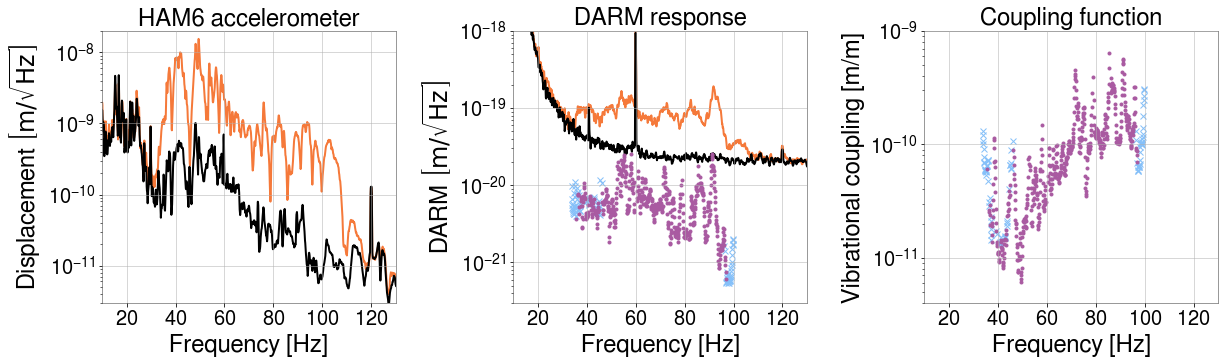
\includegraphics[width=\textwidth]{figures/ham6-injection.png}
	\caption{
		Vibrational coupling excited by a broadband (60-200\,Hz) acoustic injection near the output arm of the interferometer (HAM5 and HAM6 in Figure~\ref{fig:sensors}).
		The left plot shows the displacement of an accelerometer in the \ac{PSL} room during background time (black) and injection time (orange).
		The middle plot shows the interferometer readout during background time (black) and injection time (orange).
		Estimated ambient levels for the accelerometer are also shown as dark blue dots, with upper limits shown as light blue crosses; they are produced from the single-injection coupling function in the right plot.
		A vibrational single-injection coupling function represents meters of differential test mass displacement per meter of sensor displacement, hence the units of m/m.}
	\label{fig:injection}
\end{figure}

\begin{figure}
	\centering
	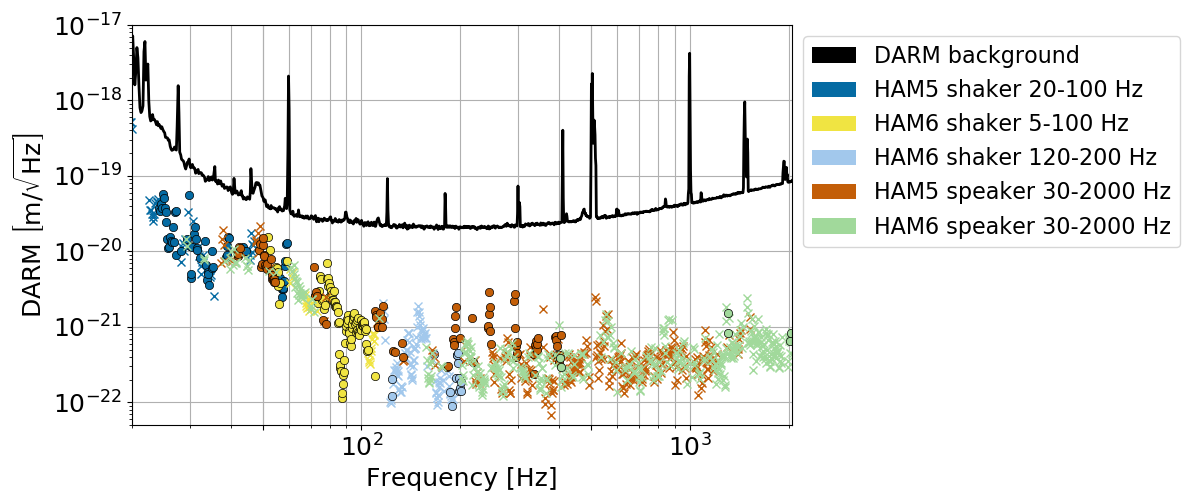
\includegraphics[width=\textwidth]{figures/composite.png}
	\caption{
		Ambient noise level for the \ac{LHO} HAM6 Y-axis accelerometer estimated from a composite coupling function, using acoustic and seismic injections near the output arm.
		For simplicity only five injections were used to produce this example, however in practice the number of injections performed near a sensor can be many times higher.}
	\label{fig:composite}
\end{figure}

\subsection{Uncertainties and limitations of coupling functions}\label{subsec:uncertainties}

\subsubsection{Comparison to transfer functions}

Environmental coupling is characterized using coupling functions instead of transfer functions because perfect coherence is not assumed in the system.
Low coherence can arise either due to non-linearity in the coupling or due to the spacing between the sensor and coupling site.
On a superficial level, a coupling function lacks a phase response component, representing only the magnitude response in the system.
Coupling functions also differ fundamentally from transfer functions in the sense that they do not assume the input signal to be the true actuation signal, but rather merely a witness of the actuation, while the actuation is in fact occurring at the location of the true coupling site.

\subsubsection{Assumptions about coupling mechanisms}

Equation~\ref{eq:cf} relies on two assumptions about the coupling mechanism.
First, the coupling is assumed to be linear in amplitude, e.g. doubling the amplitude of the injection would double the amplitude of the \ac{GW} detector response.
This is confirmed when performing injections by repeating them with different amplitudes and ensuring that the detector response scales proportionally with the injection amplitude.
Second, the coupling function ignores any up- or down-conversion of the signal between the sensor and the \ac{GW} detector.
Such non-linear coupling can be very significant for scattering noise and bilinear coupling, but is not accounted for in the estimates of linear coupling.
One way to check for non-linear coupling is by sweeping single frequency injections over time and searching for off-frequency responses in the \ac{GW} detector.
Frequency changes from non-linear coupling can be an issue in broadband injections where up- or down-converted noise in the interferometer readout appears in the injection band, resulting in artificially higher estimates at those frequencies.
We split broadband injections into smaller frequency bands to avoid this effect when necessary.
One approach for quantifying non-linear coupling is presented in Washimi et al.\ (2020)~\cite{Washimi_2020}.

\subsubsection{Hardware limitations}

\textit{Amplitude limitations}. To measure coupling, we inject signals large enough to produce a response in the detector, but the maximum amplitude of injections is limited by the sensitive range of the environmental sensors (saturation produces an overestimate of coupling).
This effectively limits how far below the detector noise background we can probe for coupling or establish upper limits.

\textit{Uncertainty due to injection locations}.
As mentioned above, the model in Equation~\ref{eq:cf_full} relies on the assumption that the environment is monitored at the coupling site.
The density of sensors is not great enough for this to be strictly true, especially if the source of the environmental signal is closer to the coupling site than the sensor is.
The detector response to an injection depends on the distance between the injection and coupling site, whereas the sensor response depends on the distance between the injection and sensor.
Varying the injection location therefore varies the relative scaling of the numerator and denominator of Equation~\ref{eq:sicf}, affecting the measurement of $\mathcal{C}_{ij}(f)$ and subsequently the sensor coupling function via Equation~\ref{eq:ccf}.
Therefore, a finite spacing of sensors leads to some degree of uncertainty in the coupling functions.
This uncertainty also propagates to projected noise levels in the \ac{GW} channel using these coupling functions.

\begin{figure}
	\centering
	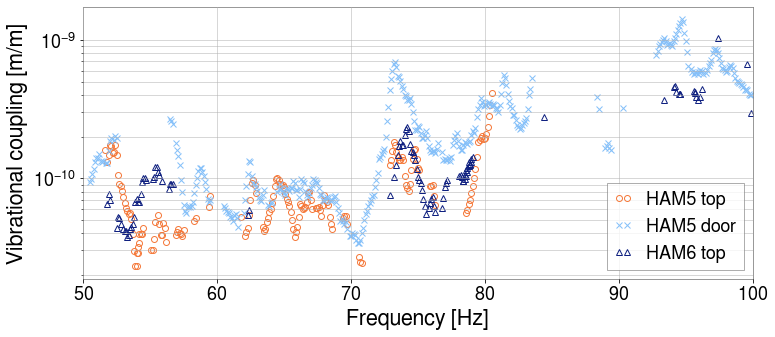
\includegraphics[width=\textwidth]{figures/injection-locations.png}
	\caption{Single-injection coupling functions (upper limits not shown) for the HAM5 Y-axis accelerometer from shaking injections made from three different locations (on top of HAM5, on top of HAM6, and on the HAM5 chamber door) show the typical spread in coupling that results from varying the injection location. Multiple injections at different frequency bands are shown for each source location. On average the coupling measured from different locations varies by a 1.4.}
	\label{fig:injection_locations}
\end{figure}

Since the uncertainty manifests as a multiplicative scaling of $\mathcal{C}_{ij}(f)$, it can be described by computing a geometric standard deviation of $\mathcal{C}_{ij}(f)$ for a single sensor over a range of injection locations, at each frequency bin.
Figure~\ref{fig:injection_locations} shows single-injection coupling functions for an accelerometer measured from shaker injections produced from three locations (the distribution of injection locations is discussed in Section~\ref{subsec:injections}.
Since the injection locations are close enough to the accelerometer, it can be assumed that the variance is primarily due to finite spacing effect.
Averaged across all frequency bins, the geometric standard deviation between injection locations is 1.4, i.e. coupling functions measured from vibrational injections can be expected to vary by a factor of 1.4 when measured by different injection locations.

A similar study was performed combining geometric standard deviations for various magnetometers at both observatories.
There are fewer magnetic injection locations to use for the comparison, but since coupling can be measured at each station (a corner station and both end stations) at each of the two LIGO observatories, there are twelve magnetometers that can be used, each with two or more injections nearby.
The result of this study is that magnetic coupling measurements and noise projections vary by a factor of 1.7~\cite{cf_uncertainty}.
This is slightly greater than that of vibrational measurements, since the lower number of magnetometers means that the distances between coupling sites and sensors is greater, amplifying the finite spacing effect.

For both vibrational and magnetic coupling, these estimated uncertainties are acceptable given that conclusions made from coupling functions are often more qualitative than strictly quantitative, i.e. identifying and localizing coupling mechanisms is more important that precise estimates of the detector response.
That said, more precise noise estimates may become important for quantifying the impact of environmental transients on \ac{GW} event candidates, as discussed in Section~\ref{subsec:vetting}.

\textit{Nodal artifacts from acoustic injections}.
In the case of acoustic injections, the uncertainty in a coupling function can be exacerbated when nodes and anti-nodes in the acoustic signal coincide with the location of a sensor but not a coupling site.
This results in peaks and troughs in the sensor spectrum at frequencies that have a node or anti-node at the sensor location, respectively.
These artifacts can impact any sensor, but are more noticeable in microphone spectra than accelerometer spectra, possibly because the stiffness of the vacuum enclosure results in effectively averaging over a larger area; in microphones, the peak-to-trough ratio is typically a factor of a few.
The peaks and troughs are present in the sensor but not in the detector spectrum, because the sensor monitors a single point whereas the coupling to the interferometer is spread across a large enough area for the effects of nodes and anti-nodes to average out.
Consequently, this effect imprints troughs and peaks onto the coupling function.

The artifacts can be smoothed out of the spectra by applying a moving average over $x_{ij,\mathrm{inj}}(f)$ before computing $\mathcal{C}_{ij}(f)$.
The moving average window must be on the scale of a few Hz since this is typically the scale of the peak-to-peak distances.
On the other hand, smoothing of spectra can also result in less accurate coupling measurements when narrow mechanical resonances are present, so the window must balance the smoothing of artifacts against this disadvantage.
For accelerometer spectra, analyzing injections with various smoothing parameters show that a logarithmically-scaled window which is \XX\,Hz wide at 100\,Hz and \XX\,Hz wide at 1000\,Hz best satisfy these constraints.
Since microphones are much more sensitive to nodal artifacts while being less sensitive to narrow mechanical resonances (they would have to be strong enough to produce audible signals), their spectra can be smoothed much more aggressively: a logarithmically-scaled window is used which is 15\,Hz wide at 100\,Hz and 150\,Hz wide at 1000\,Hz.

\subsection{Tests of coupling functions}

Although the injections used to measure coupling functions are designed to best replicate environmental noise, there are still differences and it is useful to test the coupling functions with different environmental events by comparing noise seen in the \ac{GW} strain data during such events to noise levels predicted by PEM sensors and their coupling functions.
Thunderstorms are known to produce short-duration transients in the strain data at tens of Hz.
At \ac{LLO}, coupling functions for several accelerometers at the Y end station, where vibrational coupling was the highest, are capable of estimating the amplitude of multiple noise transients to within a factor two during a particularly loud thunderstorm~\cite{alog_thunder}.
Helicopter flyovers can produce narrow-band features up to tens of seconds long.
Coupling functions of various sensors at both observatories can predict the amplitudes of lines produced by multiple helicopter flyovers during O3 to within a factor of two in most cases~\cite{alog_helicopter}.
Long-duration noise due to vibrations from rain and the building \ac{HVAC} is also well characterized by coupling functions at \ac{LHO}~\cite{alog_rain, alog_hvac_coupling}.

\subsection{The \pemcoupling package}

This section covers the technical details of the \pemcoupling python package, which includes command-line tools for processing large numbers of injections and producing single-injection coupling functions, composite coupling functions, and multi-channel summary coupling functions.

The package uses the \code{gwpy} library for fetching raw time series data and producing \acp{ASD} of the \ac{GW} strain channel and auxiliary channels from user-provided background and injection times.

Preprocessing of the time series and spectra is done mainly using \code{numpy} functions.

For each single-injection coupling function, the data are saved in the following forms:
\begin{enumerate}
	\item comma-separated text file consisting of data as described in Table~\ref{tab:pemcoupling_format}
	\item plot of the  raw coupling function (units of meters per analog-to-digital counts)
	\item plot of the coupling function in physical units (meters per calibrated sensor unit, e.g. Tesla for magnetometers)
	\item figure containing two subplots: one showing the background and injection spectra of the auxiliary sensor, and one showing the background and injection spectra of the \ac{GW} strain data and the estimated environmental noise projection.
\end{enumerate}

\begin{table}\label{tab:pemcoupling_format}
	\renewcommand{\arraystretch}{1.5}
	\begin{tabular}{|ll|}
		\hline
		\multicolumn{1}{|l}{\textbf{column}} & \multicolumn{1}{l|}{\textbf{description}}                             \\ \hline
		frequency      & bin center frequency {[}Hz{]}                                                               \\
		factor         & coupling factor in {[}m/calibrated sensor unit{]}                                           \\ 
		factor\_counts & coupling factor in {[}m/ADC count{]}                                                        \\ 
		flag           & ``Measured", ``Upper Limit", ``Thresholds not met", or ``No data"                           \\ 
		sensINJ        & sensor amplitude at injection time {[}calibrated sensor unit $\cdot\,\rthz${]}              \\ 
		sensBG         & sensor amplitude at background time {[}calibrated sensor unit $\cdot\,\rthz${]}             \\ 
		darmINJ        & \ac{GW} channel amplitude at injection time $[\meter\,\rthz]$                                    \\ 
		darmBG         & \ac{GW} channel amplitude at background time $[\meter\,\rthz]$                                   \\ \hline
	\end{tabular}
	\caption{Column descriptions for the single-injection coupling function output of the \pemcoupling package.}
\end{table}

\subsection{Environmental noise in the third LIGO/Virgo observing run}

\subsection{Validation of gravitational wave event candidates}\label{subsec:vetting}
